\begin{frame}[label=performance]
    \frametitle{Understanding a Network's Performance}
    \begin{columns}
        \begin{column}[c]{0.6\textwidth}
            How can we know what meteors are NOT seen? 
            \begin{center}
                \uncover<2->{~ \(\qquad \xrightarrow[]{}\)Through \alert{simulation!}}
            \end{center}
            \begin{enumerate}
                \setbeamertemplate{enumerate item}{\alert{Step \arabic{enumi}:}}
                \item<3-> Generate a representative population of meteors
                \item<4-> For every \textcolor{blue}{\textbf{TX}} site, calculate the power reflected off each meteor towards each \textcolor{red}{\textbf{RX}}
                \item<5-> Investigate which meteor reflect enough power to be observed by each \textcolor{blue}{\textbf{TX}}-\textcolor{red}{\textbf{RX}} link
            \end{enumerate} 

            \uncover<6->{This is the \alert{Monte Carlo method} of investigation
            \begin{itemize}
                \item[\textcolor{green}{\checkmark}] \textcolor{green}{\textit{Pros}}: Investigate complex systems through many simple simulations
                \item[\textcolor{red}{\(\times\)}] \textcolor{red}{\textit{Cons}}: Requires the simulation of many, many meteors to be useful!
            \end{itemize}}
        \end{column}
        \begin{column}[c]{0.4\textwidth}
            \centering %
            \includegraphics<3>[width=\linewidth]{img/gen_sim.pdf}%
            \includegraphics<4>[width=\linewidth]{img/full_sim.pdf}%
            \includegraphics<5>[width=\linewidth]{img/visible_sim.pdf}%
            \only<6->{\vspace*{0.2cm}
            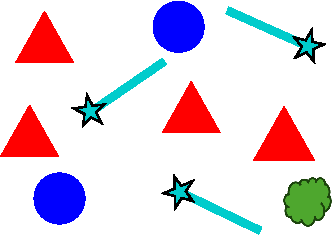
\includegraphics[height=2cm]{img/gen_sim.pdf} 
            \vspace*{0.2cm}
            
            \uncover{\hrule{}} \vspace*{0.2cm}
            \includegraphics<4->[height=2cm]{img/full_sim.pdf} 
            \vspace*{0.2cm}

            \uncover{\hrule{}} \vspace*{0.2cm}
            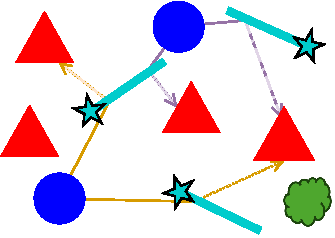
\includegraphics[height=2cm]{img/visible_sim.pdf}}
        \end{column}
    \end{columns}
\end{frame}